\documentclass[11pt]{article}
\usepackage[a4paper,margin=25mm]{geometry}
\usepackage{amsmath,amssymb,mathrsfs,graphicx}
\usepackage[unicode,colorlinks=true,urlcolor=blue,linkcolor=blue]{hyperref}
\usepackage{microtype}
\setlength{\emergencystretch}{3em}
\title{The original zeta endpoint, the heat range, and the arithmetic prime class}
\author{Split-Zero research programme}
\date{23 September 2026}
\begin{document}
\maketitle
\noindent
The positive-time theta filter has no tempered preimage of the actual
theta heat function. Its missing range component is exactly the class
of the endpoint constant \(1/16\), fixed by the residue of the original
zeta function. This note proves the full Schwartz range and inverse,
constructs a faithful source retaining the two endpoint continuations,
and evaluates the resulting prime-boundary class. It then gives an
invertible source filter and the complete original-zeta arithmetic
pairing for that test. No sign of that final pairing is assumed.
\begin{figure}[ht]
\centering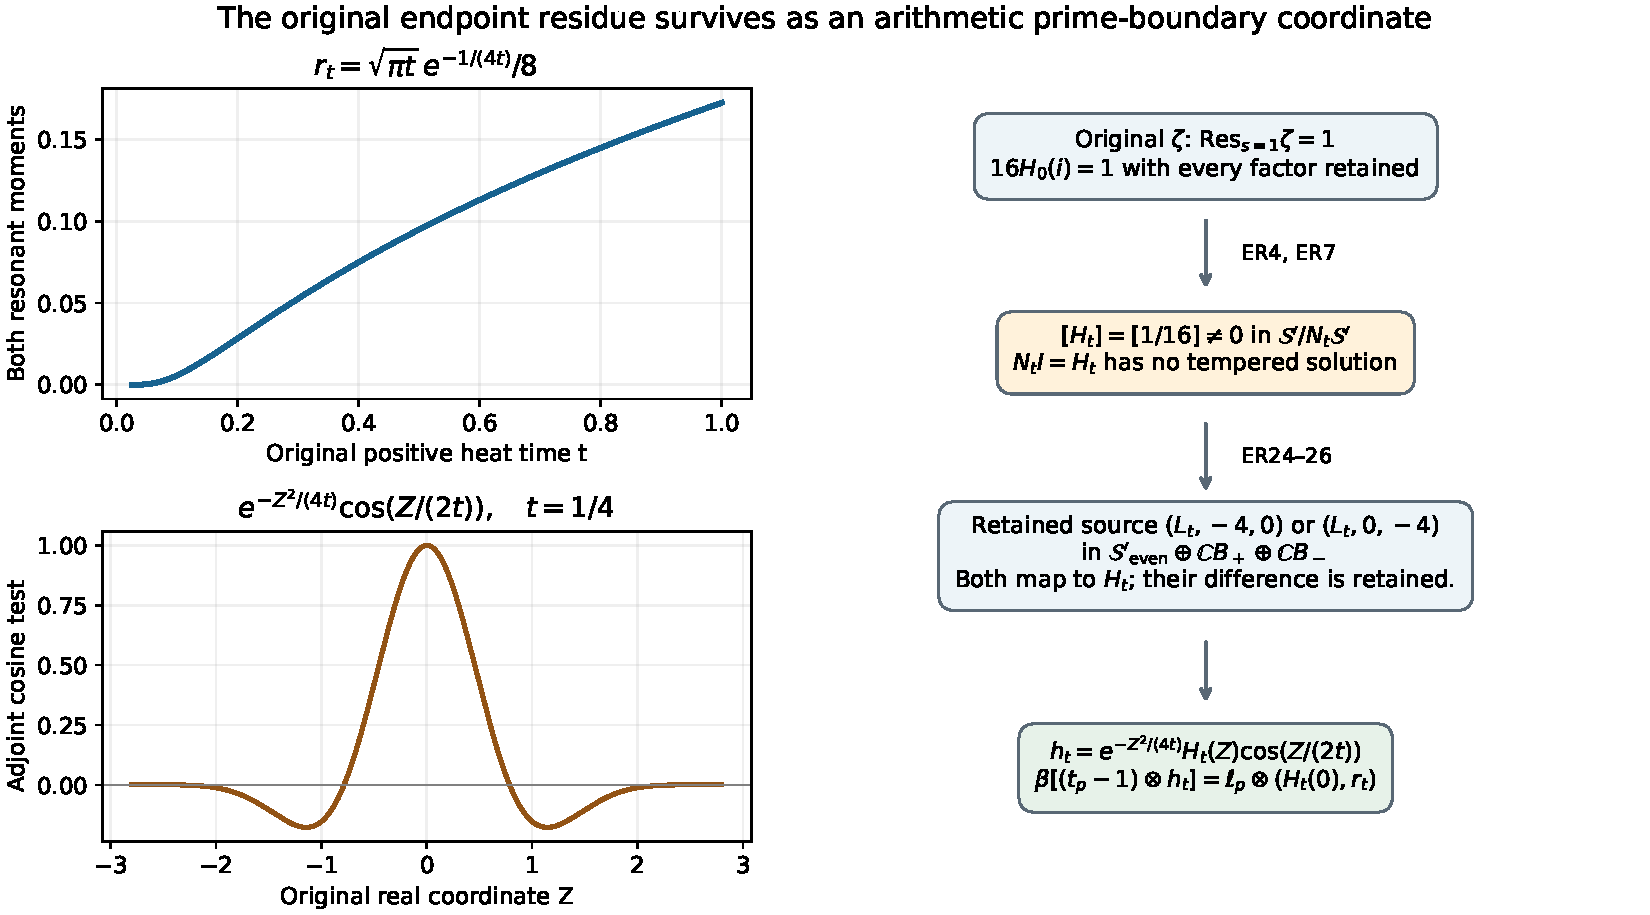
\includegraphics[width=\linewidth]{ENDPOINT_RESONANCE.pdf}
\caption{Exact moments ER7 and an adjoint test at the stated original
time, with the maps proved in ER21, ER24--30. The last arrow constructs
the displayed Schwartz test from \(H_t\); it does not identify a
distribution source with its arithmetic quotient. The human theta
source is Rodgers--Tao, equations \texttt{hoz}, \texttt{sas},
\texttt{phidef}, \texttt{htdef}; the arithmetic periodization source is
Connes, Section III (6)--(19), as cited in the proof. The plotted
curves are the exact displayed functions, not computed zero data.}
\end{figure}
\section{The missing heat endpoint is detected by the original arithmetic residue}
\label{sec:endpoint-resonance}

We calculate a range obstruction, its exact inverse on the range, and a
faithful enlarged source. The obstruction has an evaluated value fixed
by the residue of the original Riemann zeta function. It also determines
a nonzero class in the existing prime-boundary quotient. All calculations
use the original coordinate \(s=\tfrac12+iZ/2\), the original time \(t\),
and the complete multiplier
\[
 C(s)=s(s-1)\pi^{-s/2}\Gamma(s/2).
 \tag{ER1}
\]
The relevant source is Brad Rodgers and Terence Tao,
\href{https://arxiv.org/abs/1801.05914v5}{\emph{The de Bruijn--Newman
constant is non-negative}}, original author TeX, equations
\texttt{hoz}, \texttt{sas}, \texttt{phidef}, and \texttt{htdef}.
We use its exact theta density and prove the new range and receiving
statements below. No assumption about the location of nontrivial zeros
enters this calculation.

\subsection{The exact resonant moments}

Write
\[
 \Phi(u)=\sum_{n\geq1}
 (2\pi^2n^4e^{9u}-3\pi n^2e^{5u})e^{-\pi n^2e^{4u}},
 \qquad H_t(Z)=\int_0^\infty e^{tu^2}\Phi(u)\cos(Zu)\,du .
 \tag{ER2}
\]
Poisson summation gives the even extension of \(\Phi\). Every derivative
of this extension decreases faster than any Gaussian at both ends.
One can verify the latter assertion directly on \(u\geq0\) by
termwise differentiation of ER2: every differentiated term is a
polynomial in \(n^2e^{4u}\) times fixed exponentials in \(u\) and
\(e^{-\pi n^2e^{4u}}\); its sum has the asserted bound.
Evenness gives the assertion on \(u\leq0\). Thus \(H_t\) restricted
to the real \(Z\)-axis is Schwartz for every real \(t\), by repeated
integration by parts in the whole-line Fourier integral of the even
density. It is also entire in \(Z\).

The original theta identity is
\[
 16H_0(-2i(s-\tfrac12))=C(s)\zeta(s).
 \tag{ER3}
\]
Here every product at an exceptional point means its meromorphic
continuation with both factors retained. In particular
\[
 \lim_{s\to1}(s-1)\zeta(s)=1,\quad
 \lim_{s\to1}\frac{C(s)}{s-1}
 =1\cdot\pi^{-1/2}\Gamma(1/2)=1,\quad H_0(i)=\frac1{16}.
 \tag{ER4}
\]
These limits also follow from the full theta formula
\[
 \pi^{-s/2}\Gamma(s/2)\zeta(s)
 =-\frac1s+\frac1{s-1}
 +\int_1^\infty\psi(x)
   \{x^{s/2-1}+x^{(1-s)/2-1}\}\,dx,\quad
 \psi(x)=\sum_{n\ge1}e^{-\pi n^2x}.
 \tag{ER5}
\]
The integral is entire, with locally uniform derivative convergence.
Consequently the residue in ER4 is an original endpoint contribution,
not a substituted hypothesis about a completed function.

For \(t>0\), put
\[
 \omega_t=\frac1{2t},\qquad
 \ell_{\pm,t}(h)=\int_{\mathbb R}
 e^{-Z^2/(4t)}e^{\pm iZ/(2t)}h(Z)\,dZ .
 \tag{ER6}
\]
For tempered distributions these integrals mean the complex-bilinear
distribution pairing with the displayed Schwartz test, with no
conjugation. Gaussian integration gives
\[
 \boxed{\ell_{+,t}(H_t)=\ell_{-,t}(H_t)
 =2\sqrt{\pi t}\,e^{-1/(4t)}H_0(i)
 =\frac{\sqrt{\pi t}}8e^{-1/(4t)}=:r_t>0.}
 \tag{ER7}
\]
Indeed the inner Gaussian integral against \(\cos(Zu)\) is
\[
 \sqrt{\pi t}
 \{e^{-t(u+\omega_t)^2}+e^{-t(u-\omega_t)^2}\}
 =2\sqrt{\pi t}\,e^{-tu^2-1/(4t)}\cosh u.
 \tag{ER8}
\]
Fubini is justified by the finite integral of
\(e^{tu^2}|\Phi(u)|\) times the absolute Gaussian integral.
Multiplication by the retained \(e^{tu^2}\) in ER2 yields ER7.
Thus neither the heat time nor the endpoint factor has been dropped.

\subsection{An exact range theorem on the original real axis}

Keep the full differential filter
\[
 N_t=-\frac{1+(Z-2t\partial_Z)^2}{64}
 =-\frac{1+Z^2-2t-4tZ\partial_Z+4t^2\partial_Z^2}{64}.
 \tag{ER9}
\]
It acts continuously on both \(\mathcal S(\mathbb R)\) and
\(\mathcal S'(\mathbb R)\). For the bilinear distribution pairing its
transpose is
\[
 N_t^{\mathsf T}=-\frac{1+(Z+2t\partial_Z)^2}{64},\qquad
 N_t^{\mathsf T}
 \big(e^{-Z^2/(4t)}e^{\pm iZ/(2t)}\big)=0.
 \tag{ER10}
\]
The last equality follows already from
\((Z+2t\partial_Z)e^{-Z^2/(4t)}e^{\pm iZ/(2t)}
 =\pm i e^{-Z^2/(4t)}e^{\pm iZ/(2t)}\).
Therefore \(\ell_{\pm,t}(N_tI)=0\) for every tempered \(I\).
ER7 proves
\[
 \boxed{\text{There is no }I\in\mathcal S'(\mathbb R)
                  \text{ with }N_tI=H_t,\quad t>0.}
 \tag{ER11}
\]
This is a statement about a specified map and domain.

The precise Schwartz range is
\[
 0\longrightarrow\mathcal S(\mathbb R)
 \xrightarrow{N_t}\mathcal S(\mathbb R)
 \xrightarrow{(\ell_{+,t},\ell_{-,t})}\mathbb C^2
 \longrightarrow0.
 \tag{ER12}
\]
We prove exactness and give an inverse on the first image.
For \(h\in\mathcal S\) with both moments zero, set
\[
 (\mathcal G_th)(Z)
 =-\frac{32}{t}e^{Z^2/(4t)}
   \int_{-\infty}^Z
   \sin\!\frac{Z-y}{2t}\,e^{-y^2/(4t)}h(y)\,dy .
 \tag{ER13}
\]
Twice differentiating the absolutely convergent integral proves
\(N_t\mathcal G_th=h\).
For clarity, after the exact substitution
\(g=e^{-Z^2/(4t)}I\), the equation is
\[
 g''+\frac{g}{4t^2}
       =-\frac{16}{t^2}e^{-Z^2/(4t)}h.
 \tag{ER14}
\]
The coefficient in ER13 is the coefficient in ER14 divided by
\(\omega_t\). Since both moments vanish, the full-line sine integral
vanishes for each \(Z\). On \(Z>0\) ER13 can therefore be written
using minus the complementary integral from \(Z\) to \(+\infty\).
For either sign of \(Z\), with \(|Z|\ge1\), this gives
\[
 (\mathcal G_th)(Z)=
 -\frac{32}{t}\int_0^\infty
 \sin\!\frac{v}{2t}\,
 e^{-|Z|v/(2t)-v^2/(4t)}
 h(Z+\operatorname{sgn}(Z)v)\,dv .
 \tag{ER15}
\]
Every derivative is bounded by a finite sum of the derivatives of
\(h\) times powers of \(v\), with the same exponential majorant.
For every integer \(j\ge0\),
\(\int_0^\infty v^j e^{-|Z|v/(2t)}dv
 =j!(2t/|Z|)^{j+1}\).
Together with
\(1+|Z+\operatorname{sgn}(Z)v|\ge1+|Z|\),
this proves all Schwartz estimates, with each output seminorm bounded
by finitely many input seminorms. The integral on a bounded interval
has the same property by Gaussian domination. Hence
\(\mathcal G_t:\ker(\ell_+,\ell_-)\to\mathcal S\) is continuous.

The homogeneous equation ER14 has the complete distribution solution
\(g=c_+e^{iZ/(2t)}+c_-e^{-iZ/(2t)}\). This can be proved by
factoring the constant-coefficient differential operator into its two
distinct first-order factors and solving each distribution equation
by an integrating factor. Consequently every homogeneous \(I\) is
\[
 I=e^{Z^2/(4t)}
       (c_+e^{iZ/(2t)}+c_-e^{-iZ/(2t)}).
 \tag{ER16}
\]
No nonzero such function defines a tempered distribution. To prove
this without an unsupported growth criterion, the parenthesized
function \(p(Z)\) is periodic and nonzero on an interval. Choose a
nonnegative compact smooth function \(\chi\) on such an interval.
Translate \(\chi\overline p\) by integer multiples of the period
\(4\pi t\). The pairing with ER16 is the integral of
\(e^{Z^2/(4t)}\chi|p|^2\), which grows faster than any polynomial
in the translation parameter, whereas every Schwartz seminorm of
these translated tests grows at most polynomially. This contradicts
tempered continuity. Thus \(N_t\) is injective even on \(\mathcal S'\).

Finally, the moment map is onto. For
\[
 \varphi_t(Z)=e^{-Z^2/(4t)},\qquad
 A_t=\sqrt{2\pi t}\,e^{-1/(8t)}
\]
direct Gaussian differentiation gives
\[
 \ell_{\pm,t}(a\varphi_t+bZ\varphi_t)
          =A_t(a\pm ib/2).
 \tag{ER17}
\]
For a requested pair \(u_+,u_-\), take
\(a=(u_++u_-)/(2A_t)\) and
\(b=(u_+-u_-)/(iA_t)\).
This proves ER12, including a specified continuous right inverse.
On the original even source the exact sequence instead has
\(\mathcal S_{\rm even}\), \(\mathcal S_{\rm even}\), and
\(\mathbb C\), with its last map \(\ell_{+,t}=\ell_{-,t}\).

In particular, without suppressing the complementary term,
\[
 H_t=N_t I_t^{\rm Sch}
       +\frac{e^{-1/(8t)}}{8\sqrt2}\,\varphi_t,\qquad
 I_t^{\rm Sch}=
 \mathcal G_t\!\left(H_t-
              \frac{e^{-1/(8t)}}{8\sqrt2}\varphi_t\right).
 \tag{ER18}
\]
This is the explicitly chosen Gaussian section of ER12; it is not
declared to be a unique choice of section.

\subsection{The original endpoint gives a faithful enlargement}

The actual theta density before filtering is
\(\rho(u)=8e^u\psi(e^{4u})-4e^{-u}\).
Put
\[
 L_t(Z)=8\int_0^\infty e^{tu^2+u}\psi(e^{4u})\cos(Zu)\,du .
 \tag{ER19}
\]
Every derivative of \(L_t\) is bounded on the real axis, by absolute
integration of its differentiated density. It defines a tempered
distribution. Integration by parts with all zero-endpoint terms gives
\[
 N_tL_t=H_t-\frac1{16}.
 \tag{ER20}
\]
For completeness the theta-only density in ER19 has derivative
\(-4\) at zero: differentiating Poisson reflection gives
\(\psi'(1)=-\psi(1)/4-1/8\).
For any suitable density \(r\), the full calculation is
\[
 \int_0^\infty e^{tu^2}(r''-r)\cos(Zu)\,du
       =-r'(0)-[1+(Z-2t\partial_Z)^2]
                    \int_0^\infty e^{tu^2}r\cos(Zu)\,du .
\]
The interior density for ER19 is \(64\Phi\). Substitution yields
ER20, including its sign. Thus the exact nonzero quotient class is
\[
 [H_t]=[1/16]\ne0
       \quad\hbox{in }\mathcal S'/N_t\mathcal S'.
 \tag{ER21}
\]
No general dimension assertion about this distribution quotient
is required here. The equality and its nonvanishing are fully evaluated.

Here are the actual two endpoint continuations. For \(q>0\) set
\[
 F(q,a)=\frac{\sqrt\pi}{2\sqrt q}e^{a^2/(4q)}
               \operatorname{erfc}\!\frac{a}{2\sqrt q},\qquad
 B(q,Z)=\frac{F(q,1-iZ)+F(q,1+iZ)}2.
 \tag{ER22}
\]
They equal their Gaussian integrals by completing the square.
Use the square root positive for positive \(q\), and approach
\(q=-t\) from its upper or lower half-plane to obtain \(B_+\) and
\(B_-\). The entire identity
\(\operatorname{erfc}(z)+\operatorname{erfc}(-z)=2\)
gives
\[
 B_+-B_-=-i\sqrt{\frac\pi t}
          e^{(Z^2-1)/(4t)}\cos\!\frac{Z}{2t},\qquad
 N_tB_\pm=-\frac1{64}.
 \tag{ER23}
\]
The second equation first follows for \(q=-t>0\) from the retained
endpoint derivative \((e^{-u})'(0)=-1\); analytic continuation
gives both lateral values. This is the erfc convention of
N. M. Temme, \href{https://dlmf.nist.gov/7.2.E2}{DLMF 7.2.2}.

Define a precise enlarged even source, as a subspace of distributions,
by the map
\[
 \iota_t:\mathcal S'_{\rm even}\oplus\mathbb C^2\longrightarrow
             \mathcal D'_{\rm even},\qquad
 (U,c_+,c_-)\longmapsto U+c_+B_++c_-B_- .
 \tag{ER24}
\]
This map is injective. Indeed, if the last two terms are tempered,
apply \(N_t\) and ER10. The nonzero moments of the constant show
\(c_++c_-=0\). ER23 and the translated-test proof following
ER16 then give \(c_+=c_-=0\). Its filter is exactly
\[
 N_t\iota_t(U,c_+,c_-)=N_tU-\frac{c_++c_-}{64}.
 \tag{ER25}
\]
Its kernel has precisely the one-dimensional coordinate line
\((0,c,-c)\): necessity follows again from ER10 and the injectivity
of \(N_t\) on \(\mathcal S'\); sufficiency follows from ER23.
The two original unfiltered continuations are the distinct vectors
\[
 I_+=\iota_t(L_t,-4,0),\qquad
 I_-=\iota_t(L_t,0,-4),\qquad N_tI_\pm=H_t.
 \tag{ER26}
\]
They satisfy the heat equation on their actual sectorial domains
by differentiating the convergent integral for negative time and
continuing analytically. The enlarged source has retained, rather
than identified, both endpoint values. The full original-zeta
returns are \(I_\pm/\{\pi^{-s/2}\Gamma(s/2)\}\) and
\(16H_t/C(s)\), at \(Z=-2i(s-\tfrac12)\). Their exact map is
the filter ER9 with these displayed factors, including its derivative
terms; no equality between the two returned families is asserted.

\paragraph{The boundary values remember the chosen continuation.}
For an actual solution \(I\) of \(N_tI=H_t\), let
\(g=e^{-Z^2/(4t)}I\). For \(\varepsilon=\pm1\) the complete
Green boundary is
\[
 \begin{split}
 W_\varepsilon[I](Z)
 &=e^{\varepsilon iZ/(2t)}
                  [g'(Z)-\varepsilon i g(Z)/(2t)]\\
 &=e^{-Z^2/(4t)}e^{\varepsilon iZ/(2t)}
       \left[I'(Z)-\left(\frac{Z}{2t}
                    +\frac{\varepsilon i}{2t}\right)I(Z)\right],\\
 W_\varepsilon[I]'(Z)
 &=-\frac{16}{t^2}e^{-Z^2/(4t)}
                       e^{\varepsilon iZ/(2t)}H_t(Z).
 \end{split}
 \tag{ER26a}
\]
The last identity follows from ER14 by differentiation.
Equivalently, integration of the full original differential operator
over \([a,b]\) gives
\[
 \int_a^b(\psi_\varepsilon N_tI-
                    I N_t^{\mathsf T}\psi_\varepsilon)\,dZ
 =-\frac{t^2}{16}[W_\varepsilon[I]]_a^b,
 \quad \psi_\varepsilon=e^{-Z^2/(4t)}e^{\varepsilon iZ/(2t)} .
 \tag{ER26b}
\]
The drift term contributes \(-Z\psi_\varepsilon I/t\) inside
the second-derivative Green bracket
\(\psi_\varepsilon I'-\psi_\varepsilon'I-Z\psi_\varepsilon I/t\).
Inserting \(\psi_\varepsilon'\) gives exactly ER26b.
The right side of ER26a is integrable on the real line. Both
Wronskian limits exist, and their difference is
\[
 W_\varepsilon(+\infty)-W_\varepsilon(-\infty)
       =-2\sqrt{\pi}\,t^{-3/2}e^{-1/(4t)}.
 \tag{ER26c}
\]

The separate limits can also be calculated. Write
\(c_t=\sqrt{\pi/t}\,e^{-1/(4t)}\). Direct substitution
in ER22 on the upper \(q\)-branch gives
\[
 \begin{split}
 e^{-Z^2/(4t)}I_+
 ={}&e^{-Z^2/(4t)}L_t\\
 &+ic_t\left\{
 e^{iZ/(2t)}\operatorname{erfc}\frac{-Z-i}{2\sqrt t}
 +e^{-iZ/(2t)}\operatorname{erfc}\frac{Z-i}{2\sqrt t}
 \right\}.
 \end{split}
 \tag{ER26d}
\]
For \(x>0\) and fixed real \(y\),
\[
 \operatorname{erfc}(x+iy)
  =\frac2{\sqrt\pi}\int_x^\infty e^{-(v+iy)^2}dv,\qquad
 |\operatorname{erfc}(x+iy)|
        \le\frac{e^{y^2-x^2}}{\sqrt\pi x}.
\]
The first formula follows by moving the entire primitive to a
horizontal ray; the extra vertical segment tends to zero at infinity.
The bound follows by comparison with the real Gaussian tail.
Its derivative has the Gaussian bound from
\(\operatorname{erfc}'(z)=-2e^{-z^2}/\sqrt\pi\).
Use also \(\operatorname{erfc}(-z)=2-\operatorname{erfc}(z)\).
Since \(L_t,L_t'\) are bounded, ER26d and ER23 now show
that \(e^{-Z^2/(4t)}I_+\) tends to
\(2ic_te^{iZ/(2t)}\) at \(+\infty\) and
\(2ic_te^{-iZ/(2t)}\) at \(-\infty\), with remainders
and their derivatives tending to zero. For \(I_-\) the corresponding
terms are \(-2ic_te^{-iZ/(2t)}\) and
\(-2ic_te^{iZ/(2t)}\). Substitution into ER26a proves
\[
 \begin{array}{c|cc|cc}
 &W_+(-\infty)&W_+(+\infty)&W_-(-\infty)&W_-(+\infty)\\\hline
 I_+&2c_t/t&0&0&-2c_t/t\\
 I_-&0&-2c_t/t&2c_t/t&0 .
 \end{array}
 \tag{ER26e}
\]
Every row retains the same compulsory difference ER26c.

On the actual arithmetic line put \(A(s)=\pi^{-s/2}\Gamma(s/2)\)
and \(f_\pm(t,s)=I_\pm(t,-2i(s-\tfrac12))/A(s)\).
There \(A\) is nonzero and holomorphic. Since
\(\partial_Z=(i/2)\partial_s\), the same boundary becomes
\[
 \begin{split}
 W_\varepsilon[I_\pm]
 ={}&\exp\!\frac{(s-\tfrac12)^2+\varepsilon(s-\tfrac12)}t\\
 &\times\left\{\frac i2[A'f_\pm+A\partial_sf_\pm]
       +\frac it\left(s-\frac{1+\varepsilon}{2}\right)Af_\pm\right\},\\
 A'(s)={}&A(s)\left[-\frac{\log\pi}{2}
                              +\frac12\psi_\Gamma(s/2)\right].
 \end{split}
 \tag{ER26f}
\]
Both multiplier derivatives and both endpoint limits are retained.
This gives the exact original-zeta boundary receiving map, including
the data changed by choosing a different lateral continuation.

\subsection{An evaluated prime-boundary class and its full zeta transform}

There is an arithmetic receiver for the nonzero obstruction value.
Define the actual even Schwartz source
\[
 h_t(Z)=e^{-Z^2/(4t)}H_t(Z)\cos\!\frac{Z}{2t}.
 \tag{ER27}
\]
Its original two moments are
\[
 \left(h_t(0),\int_{\mathbb R}h_t(Z)\,dZ\right)
           =(H_t(0),r_t).
 \tag{ER28}
\]
Let \(H=\mathcal S_{\rm even}(\mathbb R)\),
\(H_0=\{h:h(0)=\int h=0\}\),
\(R=\mathbb C[\mathbb Q_{>0}^{\times}]\), and
\(I=\ker(\operatorname{aug}:R\to\mathbb C)\).
For \(M_0=\ker(\operatorname{aug}\otimes(h\mapsto(h(0),\int h)))\),
the existing quotient is \(Q_0=M_0/IM_0\).
Its exact prime-boundary coordinate is
\[
 \beta\left[\sum_a t_a\otimes h_a\right]
  =\sum_p\ell_p\otimes\sum_a v_p(a)
                \left(h_a(0),\int h_a\right).
 \tag{ER29}
\]
To recall why this is a well-defined detecting map, the functions
\((1-2\pi Z^2)e^{-\pi Z^2}\) and \(2\pi Z^2e^{-\pi Z^2}\)
have moments \((1,0)\) and \((0,1)\). They split \(H\) into
\(H_0\oplus\mathbb C^2\), so
\(M_0=(R\otimes H_0)\oplus(I\otimes\mathbb C^2)\).
Dividing by \(IM_0\) gives
\[
 Q_0=H_0\oplus(I/I^2)\otimes\mathbb C^2,\qquad
 I/I^2\cong\bigoplus_p\mathbb C\ell_p.
\]
The last isomorphism follows from
\(t_{ab}-1=(t_a-1)+(t_b-1)+(t_a-1)(t_b-1)\)
and prime factorization; the valuations \(v_p\) kill \(I^2\)
and separate the displayed generators. This proves ER29 and
the claimed detection without a new quotient assumption.

For every prime \(p\), the particular class is now evaluated:
\[
 b_{p,t}=[(t_p-1)\otimes h_t],\qquad
 \boxed{\beta b_{p,t}=\ell_p\otimes
      \left(H_t(0),\frac{\sqrt{\pi t}}8e^{-1/(4t)}\right)\ne0.}
 \tag{ER30}
\]
Its original sum-of-components map is zero. Therefore the original
periodization
\(\mathcal E(c)(x)=2x^{1/2}\sum_{n\ge1}(\Phi c)(nx)\)
and its full
\(\int_0^\infty|\mathcal E(c)(x)|^2
 (1+\log^2x)^{\delta/2}\,dx/x\), \(\delta>1\),
vanish on this class. These are the moment and periodization
conventions of
\href{https://arxiv.org/abs/math/9811068v1}{Alain Connes,
\emph{Trace formula in noncommutative geometry and the zeros of the
Riemann zeta function}}, Section III (6)--(19).
The algebraic prime quotient and its proved source comparison are
\href{https://github.com/KokunoYumeto/zeta-function-research-reader/blob/ec73ac350d0cda3d95c0bd1361bede33166b4d34/workbenches/splitzero-tandem/continuations/20260923-original-zeta-return/NOTE.tex}{FR15--25}.
No new positive norm on these zero-seminorm classes is assigned.

There is more information than these two moments. Put
\(w=s-\tfrac12\) and retain the full Mellin convention
\(\mathcal M h(s)=\int_{\mathbb R}h(Z)e^{-wZ}\,dZ\).
For every complex \(s\), the complete test is
\[
 \mathcal M h_t(s)=\sqrt{\pi t}
 \left\{e^{t(w-i/(2t))^2}H_0(2tw-i)
       +e^{t(w+i/(2t))^2}H_0(2tw+i)\right\}.
 \tag{ER31}
\]
To prove this, first omit the cosine in ER27. Gaussian integration
with the complete \(H_t\) source gives
\[
 \int_{\mathbb R}e^{-Z^2/(4t)}H_t(Z)e^{-wZ}\,dZ
        =2\sqrt{\pi t}\,e^{tw^2}H_0(2tw).
 \tag{ER32}
\]
Absolute interchange holds for every fixed complex \(w\), since
the outer Gaussian dominates \(e^{|\Re w||Z|}\), and
\(\int e^{tu^2}|\Phi(u)|du<\infty\).
The inner Gaussian formula is entire in \(w\).
The two exponentials of the retained cosine give ER31.

In terms of the original zeta function, set
\(\sigma_0=it(s-\tfrac12)\) and
\(\sigma_1=1+it(s-\tfrac12)\). ER3 gives the exact formula
\[
 \boxed{\begin{aligned}
 \mathcal M h_t(s)=\frac{\sqrt{\pi t}}{16}\big\{&
 e^{t(w-i/(2t))^2}
 \sigma_1(\sigma_1-1)\pi^{-\sigma_1/2}
       \Gamma(\sigma_1/2)\zeta(\sigma_1)\\
 {}+{}&
 e^{t(w+i/(2t))^2}
 \sigma_0(\sigma_0-1)\pi^{-\sigma_0/2}
       \Gamma(\sigma_0/2)\zeta(\sigma_0)\big\}.
 \end{aligned}}
 \tag{ER33}
\]
All endpoint factors, Gamma factors and powers of pi are shown.
Each product is continued as the product in ER3 at every zero or
pole of a factor. At \(s=1/2\), the two exceptional arguments are
exactly \(1\) and \(0\). Their products are both \(1\):
the first is ER4, and the second follows from
\(C(0)=-2\), \(\zeta(0)=-1/2\).
Substitution in ER33 reproduces \(r_t\) in ER28.
Both endpoints thus contribute to the evaluated prime-boundary
coordinate. The endpoint values \(\mathcal M h_t(0)\) and
\(\mathcal M h_t(1)\) are also the full expressions ER33 at
\(w=-1/2\) and \(w=1/2\); no endpoint-null test has been imposed.

\subsection{An invertible test filter and the complete arithmetic pairing}

The just-constructed source can be taken to an endpoint-null test
without losing its information. This requires the inverse, not merely
the assertion that the endpoint values vanish. In the same real
coordinate put
\[
 f_t=(\partial_Z^2-\tfrac14)h_t,\qquad
 F_t(s)=s(s-1)\mathcal M h_t(s),\qquad
 k_t=f_t*f_t .
 \tag{ER34}
\]
Gaussian decay of \(h_t\) and every derivative follows from ER27,
because all derivatives of \(H_t\) are bounded on the real axis.
Thus integration by parts proves
\(\mathcal M f_t=F_t\), with the two endpoints
\(F_t(0)=F_t(1)=0\) evaluated exactly. ER33 remains the full
formula for \(\mathcal M h_t\); its factors are not omitted.

The distribution \(G(Z)=-e^{-|Z|/2}\) satisfies
\((\partial_Z^2-\tfrac14)G=\delta_0\): the derivative jump
of \(e^{-|Z|/2}\) is \(-1\), fixing the sign and coefficient.
The inverse on the actual Schwartz source is
\[
 h_t(Z)=-\int_{\mathbb R}e^{-|Z-y|/2}f_t(y)\,dy .
 \tag{ER35}
\]
More generally convolution with \(G\) is continuous on Schwartz
space. Move derivatives to the Schwartz factor and use
\((1+|Z|)^M\le(1+|Z-y|)^M(1+|y|)^M\);
every polynomially weighted exponential is integrable.
The only solutions of the homogeneous differential equation
are \(ae^{Z/2}+be^{-Z/2}\), none nonzero and Schwartz.
This proves the two-sided inverse. Although the displayed convolution
permits exponential tails for a generic Schwartz input, for the
actual \(f_t\) it returns exactly the Gaussian-decaying \(h_t\);
the endpoint equalities are retained in that assertion.

The prime-boundary coordinates of this filtered source are also
fully evaluated:
\[
 \boxed{\beta[(t_p-1)\otimes f_t]
 =\ell_p\otimes\left(
 H_t''(0)-
 \left(\frac1{2t}+\frac1{4t^2}+\frac14\right)H_t(0),
 -\frac{\sqrt{\pi t}}{32}e^{-1/(4t)}
 \right).}
 \tag{ER36}
\]
Differentiate ER27 twice at zero to obtain its first entry;
integrate \(f_t\) and use \(\int h_t''=0\) for the second.
Every summand in \(\Phi(u)\) is positive on \(u\ge0\), since
\(2\pi n^2e^{4u}>3\). Hence
\[
 H_t(0)>0,\qquad
 H_t''(0)=-\int_0^\infty u^2e^{tu^2}\Phi(u)\,du<0,
\]
and both entries of ER36 are strictly negative. These are signs
of two actual source moments. They are not asserted to be signs
of the Weil quadratic form.

For completeness we give that quadratic form's exact receiving
formula, with all original arithmetic contributions. Let
\[
 \begin{split}
 j(s)&=\zeta'(s)/\zeta(s),\\
 \kappa(s)&=-\tfrac12\log\pi+\tfrac12\psi_\Gamma(s/2),\\
 A_t(s)&=F_t(s)^2,\qquad
 d_{m,t}=A_t(-2m),\qquad U_{N,t}=\sum_{m=1}^Nd_{m,t},\\
 K_t&=\sum_{\rho}m_\rho F_t(\rho)^2,\qquad
 V_{N,t}=K_t+U_{N,t}-A_t(1).
 \end{split}
 \tag{ER37}
\]
The sum in \(K_t\) is over the actual nontrivial zeros with
multiplicity. On the present real even source the reflected
test is the same \(F_t\): indeed
\(\overline{F_t(1-\bar s)}=F_t(s)\).
This proves its square in ER37 rather than replacing it by an
absolute square away from the critical line.

The Gaussian bounds for \(f_t\) and its derivatives imply Gaussian
bounds for \(k_t\) and its derivatives by convolution and
\(y^2+(x-y)^2=x^2/2+2(y-x/2)^2\).
For example fixed polynomials times \(e^{-Z^2/(4t)}\) bound
each derivative of \(f_t\); powers can be bounded by constants
times \(e^{-Z^2/(8t)}\).
Integration by parts in \(\mathcal M f_t\) then gives arbitrary
inverse-power decay on every fixed vertical strip. The original
zero count \(O(T\log(T+2))\) proves absolute convergence of
the nontrivial-zero sum. These are the same zero-count and
contour hypotheses used in the classical explicit formula.
For the human source conventions see Connes, cited above,
Appendix II (1)--(11), Theorem 1 and Theorem 6. The latter theorem
is stated for compact support. The present Gaussian source is
noncompact; the displayed Gaussian bounds and the finite-strip
argument below establish the needed extension, rather than
silently treating it as a compactly supported input.
The original reflection identity, obtained by logarithmically
differentiating ER3 and its reflection while retaining both
Gamma factors, is
\[
 j(s)+j(1-s)=-\kappa(s)-\kappa(1-s).
 \tag{ER38}
\]
Let \(I_c\) denote the upward vertical integral divided by
\(2\pi i\), take \(\sigma>1\), and \(b_N=-2N-1\).
The original argument principle on this finite-width strip gives
\[
 \begin{split}
 V_{N,t}&=I_\sigma(A_tj)-I_{b_N}(A_tj),\\
 \mathcal G_{N,t}
 &=I_{b_N}\{A_t(s)[\kappa(s)+\kappa(1-s)]\},\\
 V_{N,t}&=-P_t+\mathcal G_{N,t},\\
 \mathcal G_{N,t}&=A_\infty(k_t)+A_t(0)+U_{N,t},\\
 K_t&=A_t(0)+A_t(1)+A_\infty(k_t)-P_t .
 \end{split}
 \tag{ER39}
\]
Here the complete terms are
\[
 \begin{split}
 P_t&=2\sum_{n\ge2}\frac{\Lambda(n)}{\sqrt n}k_t(\log n),
 \quad \Lambda(p^j)=\log p,\\
 A_\infty(k)&=-(\gamma_{\rm E}+\log\pi)k(0)\\
 &\quad+\int_0^\infty
 \frac{e^{-x}k(0)-\tfrac12e^{-x/4}
               [k(x/2)+k(-x/2)]}{1-e^{-x}}\,dx,\\
 A_t(0)&=A_t(1)=0 .
 \end{split}
 \tag{ER40}
\]
Both prime legs occur in the factor two because \(k_t\) is even.
The Gamma numerator is kept together: its first-order difference
is \(O(x)\) and its symmetric second difference is \(O(x^2)\)
at zero. The Gaussian tails prove absolute convergence of the
prime sum, including all prime powers, and of the remaining
Gamma integral.

To verify ER39, exhaust the strip in height along levels avoiding
zero ordinates. The logarithmic derivative of the original function,
with the full derivative of \(C\) retained in its factored expansion,
has polynomial bounds along such a sequence; the vertical test's
arbitrary inverse-power decay kills the horizontal edges. The
enclosed original divisor is exactly the nontrivial zeros, the
first \(N\) negative even integers, and the pole at one.
Inserting ER38 on the left edge and using
\(j(s)=-\sum_{n\ge2}\Lambda(n)n^{-s}\) on the right gives
the two prime legs by Mellin inversion. Shifting the Gamma
edge to \(1/2\) crosses residues \(-1\) at
\(0,-2,\ldots,-2N\), and therefore adds precisely
\(A_t(0)+U_{N,t}\) to its value on the left.
The line \(1/2\) gives \(A_\infty\) by the original digamma
integral, whose full numerator is ER40. This proves all signs
and every finite-cutoff term. No limit of \(U_{N,t}\) is
presupposed or assigned by this calculation.

The full input to ER39 has thus been constructed: \(F_t\) is the
two-argument original-zeta expression ER33 multiplied by the
retained \(s(s-1)\), and \(k_t\) is its actual source convolution.
The map ER35 recovers the source whose prime-boundary residue
was evaluated in ER30. Formula ER39 gives its exact compensated
pairing while retaining the original signed trace, each trivial
zero and the matching Gamma boundary separately. This extension
does not claim a numerical value or sign for \(K_t\).

\paragraph{The full support carrier is retained.}
For any of the displayed complex vector spaces \(V\) and the
original bounded distributive lattice \(L\), retain the carrier
\[
 G_L(V)=\{(v,1_L):v\in V\}
       \cup\{z_\lambda=(0,\lambda):\lambda\ne1_L\},
 \quad e=(0,1_L),\quad\tau=z_{0_L}.
 \tag{ER40a}
\]
Each linear map \(A:V\to W\) proved above has the specified lift
\((v,1_L)\mapsto(Av,1_L)\), \(z_\lambda\mapsto z_\lambda\).
Composition of these lifts agrees with the lift of the composition,
and every original label is unchanged even when the amplitude
vanishes. The injective enlarged-source map ER24 remains injective
on these carriers: this follows on top amplitudes from ER24 and
on the distinct lower points from their unchanged labels.
The two different lateral inputs in ER26 have the same top-supported
image; the difference of their images has amplitude zero with label \(1_L\),
namely \(e\), rather than the absent label \(\tau\).
This construction uses the full \(L\), without replacing it by
a Boolean quotient. It is a lift of the proved linear source maps;
it does not assert that vector-space differential operators are
semiring homomorphisms, or replace the separately proved
supported-zero multiplication by an identity operator.

ER11, ER21, ER24--26 and ER30--40a give the exact relation sought:
the original arithmetic residue obstructs a tempered unfiltered
positive-time source, the two actual endpoint continuations provide
a faithful source beyond that domain, and an explicit Schwartz
receiver carries the obstruction value into the existing arithmetic
prime class and a two-argument original-zeta test. The nonzero
residue occurs independently of RH. This calculation does not
assign the sign of a compensated Weil form or locate a nontrivial
zero; those require their own evaluated arithmetic pairings.

\end{document}
